%%%%%%%%%%%%%%%%%%%%%%%%%%%%%%%%%%%%%%%%%
% Short Sectioned Assignment LaTeX Template Version 1.0 (5/5/12)
% This template has been downloaded from: http://www.LaTeXTemplates.com
% Original author:  Frits Wenneker (http://www.howtotex.com)
% License: CC BY-NC-SA 3.0 (http://creativecommons.org/licenses/by-nc-sa/3.0/)
%%%%%%%%%%%%%%%%%%%%%%%%%%%%%%%%%%%%%%%%%

% \documentclass[paper=a4, fontsize=11pt]{scrartcl} % A4 paper and 11pt font size
\documentclass[11pt, a4paper]{book}
\usepackage[T1]{fontenc} % Use 8-bit encoding that has 256 glyphs
\usepackage[utf8]{inputenc}
\usepackage{fourier} % Use the Adobe Utopia font for the document - comment this line to return to the LaTeX default
\usepackage{listings} % para insertar código con formato similar al editor
\usepackage[spanish, es-tabla]{babel} % Selecciona el español para palabras introducidas automáticamente, p.ej. "septiembre" en la fecha y especifica que se use la palabra Tabla en vez de Cuadro
\usepackage{url} % ,href} %para incluir URLs e hipervínculos dentro del texto (aunque hay que instalar href)
\usepackage{graphics,graphicx, float} %para incluir imágenes y colocarlas
\usepackage[gen]{eurosym} %para incluir el símbolo del euro
\usepackage{cite} %para incluir citas del archivo <nombre>.bib
\usepackage{enumerate}
\usepackage{hyperref}
\usepackage{graphicx}
\usepackage{tabularx}
\usepackage{booktabs}
\usepackage{pdflscape}
\usepackage{amsmath}

% \usepackage{array} % Para celdas personalizadas
% \usepackage{geometry} % Para ajustar los márgenes
% \geometry{a4paper, margin=1in}

\usepackage[table,xcdraw]{xcolor}
\hypersetup{
	colorlinks=true,	% false: boxed links; true: colored links
	linkcolor=black,	% color of internal links
	urlcolor=cyan		% color of external links
}
\renewcommand{\familydefault}{\sfdefault}
\usepackage{fancyhdr} % Custom headers and footers
\pagestyle{fancyplain} % Makes all pages in the document conform to the custom headers and footers
\fancyhead[L]{} % Empty left header
\fancyhead[C]{} % Empty center header
\fancyhead[R]{Elena Ortega Contreras} % My name
\fancyfoot[L]{} % Empty left footer
\fancyfoot[C]{} % Empty center footer
\fancyfoot[R]{\thepage} % Page numbering for right footer
%\renewcommand{\headrulewidth}{0pt} % Remove header underlines
\renewcommand{\footrulewidth}{0pt} % Remove footer underlines
\setlength{\headheight}{13.6pt} % Customize the height of the header

\usepackage{titlesec, blindtext, color}
\definecolor{gray75}{gray}{0.75}
\newcommand{\hsp}{\hspace{20pt}}
\titleformat{\chapter}[hang]{\Huge\bfseries}{\thechapter\hsp\textcolor{gray75}{|}\hsp}{0pt}{\Huge\bfseries}
\setcounter{secnumdepth}{4}
\usepackage[Lenny]{fncychap}

\definecolor{vskeywordcolor}{RGB}{86, 156, 214} % Azul para palabras clave
\definecolor{vscommentcolor}{RGB}{87, 166, 74}  % Verde para comentarios
\definecolor{vsstringcolor}{RGB}{214, 157, 133} % Rojo para cadenas de texto
\renewcommand{\lstlistingname}{Código}

\lstset{
    breaklines=true,            % Permite cortar líneas largas
    breakatwhitespace=false,    % Rompe líneas en cualquier punto, no solo en espacios
    basicstyle=\ttfamily\footnotesize,  % Define fuente de tamaño más pequeño y monoespaciada
    lineskip=-1pt,              % Reduce el espacio entre líneas
    frame=single,               % Añade un marco alrededor del código
    captionpos=b,               % Coloca el título del código abajo (opcional)
    columns=fullflexible,       % Permite ajustar el ancho de las columnas
    keepspaces=true,            % Mantiene los espacios en blanco en el código
    xleftmargin=0.5em,          % Margen izquierdo del código
    xrightmargin=0.5em,         % Margen derecho del código
    aboveskip=1em,              % Espacio vertical antes del código
    belowskip=1em,              % Espacio vertical después del código
    keywordstyle=\color{vskeywordcolor}, % Color para palabras clave
    commentstyle=\color{vscommentcolor}, % Color para comentarios
    stringstyle=\color{vsstringcolor},   % Color para cadenas de texto
    showstringspaces=false,     % No mostrar espacios en blanco en las cadenas
}

% Fuente: https://github.com/ghammock/LaTeX_Listings_JavaScript_ES6
% Definición del lenguaje JavaScript para listados
\usepackage{xcolor}
\lstdefinelanguage{JavaScript}{
  morekeywords=[1]{break, continue, delete, else, for, function, if, in,
    new, return, this, typeof, var, void, while, with},
  % Literals, primitive types, and reference types.
  morekeywords=[2]{false, null, true, boolean, number, undefined,
    Array, Boolean, Date, Math, Number, String, Object},
  % Built-ins.
  morekeywords=[3]{eval, parseInt, parseFloat, escape, unescape},
  sensitive,
  morecomment=[s]{/*}{*/},
  morecomment=[l]//,
}

\begin{document}

	% Plantilla portada UGR
	\begin{titlepage}
    \newlength{\centeroffset}
    \setlength{\centeroffset}{-0.5\oddsidemargin}
    \addtolength{\centeroffset}{0.5\evensidemargin}
    \thispagestyle{empty}
    
    \noindent\hspace*{\centeroffset}
    \begin{minipage}{\textwidth}
    
    \centering
    
\includegraphics[width=0.9\textwidth]{logos/logo_ugr.jpg}\\[1.4cm]
    
    \textsc{ \Large TRABAJO FIN DE GRADO\\[0.2cm]}
    \textsc{ GRADO EN INGENIERIA INFORMATICA}\\[1cm]
    
    {\Huge\bfseries SIGMA \\}
    \noindent\rule[-1ex]{\textwidth}{3pt}\\[3.5ex]
    {\large\bfseries Sistema Inteligente de Gestión Monetaria Automatizada }
    \end{minipage}
    
    \vspace{2.5cm}
    \noindent\hspace*{\centeroffset}
    \begin{minipage}{\textwidth}
    \centering
    
    \textbf{Autor}\\ {Elena Ortega Contreras}\\[2.5ex]
    \textbf{Director}\\ {José Manuel Soto García}\\[2cm]
    
\includegraphics[width=0.3\textwidth]{logos/etsiit_logo.png}\\[0.1cm]
    \textsc{Escuela Técnica Superior de Ingenierías Informática y de Telecomunicación}\\
    \textsc{---}\\
    Granada, Junio de 2024
    \end{minipage}
    \end{titlepage}

	% Plantilla prefacio UGR
	\thispagestyle{empty}

\begin{center}
{\large\bfseries Título \\ Subtítulo }\\
\end{center}
\begin{center}
Nombre Del Estudiante\\
\end{center}

%\vspace{0.7cm}

\vspace{0.5cm}
\noindent\textbf{Palabras clave}: \textit{software libre}
\vspace{0.7cm}

\noindent\textbf{Resumen}\\
	

\cleardoublepage

\begin{center}
	{\large\bfseries Same, but in English}\\
\end{center}
\begin{center}
	Student's name\\
\end{center}
\vspace{0.5cm}
\noindent\textbf{Keywords}: \textit{open source}, \textit{floss}
\vspace{0.7cm}

\noindent\textbf{Abstract}\\


\cleardoublepage

\thispagestyle{empty}

\noindent\rule[-1ex]{\textwidth}{2pt}\\[4.5ex]

D. \textbf{Tutora/e(s)}, Profesor(a) del ...

\vspace{0.5cm}

\textbf{Informo:}

\vspace{0.5cm}

Que el presente trabajo, titulado \textit{\textbf{Chief}},
ha sido realizado bajo mi supervisión por \textbf{Estudiante}, y autorizo la defensa de dicho trabajo ante el tribunal
que corresponda.

\vspace{0.5cm}

Y para que conste, expiden y firman el presente informe en Granada a Junio de 2018.

\vspace{1cm}

\textbf{El/la director(a)/es: }

\vspace{5cm}

\noindent \textbf{(nombre completo tutor/a/es)}

\chapter*{Agradecimientos}

Poner aquí agradecimientos...



	% Índice de contenidos
	\newpage
	\tableofcontents

	% Índice de imágenes y tablas
	\newpage
	\listoffigures

	% Si hay suficientes se incluirá dicho índice
	\listoftables 
	\newpage


	\chapter{Introducción}
En esta sección se detalla la importancia de la gestión económica personal y cómo el avance de la digitalización ha transformado la manera en que interactuamos con nuestras finanzas. Se presenta un recorrido por la evolución de los servicios financieros digitales en España, desde los primeros cajeros automáticos hasta las modernas formas de pago como \textit{Bizum} y \textit{NFC}. Asimismo, se analizan los retos actuales que enfrentan los usuarios al gestionar sus finanzas personales, dadas las múltiples fuentes de ingresos y métodos de pago disponibles. Se explora cómo las soluciones \textit{Fintech} han surgido para abordar estos desafíos.

\section{Contexto. Descripción del problema} 
Según su definición en la \href{https://dle.rae.es/economía}{RAE} la economía es la 
\textit{Administración eficaz y razonable de los bienes}, dicho esto y teniendo en 
cuenta que nos concierne a todos, es crucial tener control sobre ella. 
De manera individual, las decisiones financieras influyen en la calidad de vida de las personas,
un uso adecuado es esencial para evitar problemas como el endeudamiento, la 
falta de ahorro o la incapacidad de cumplir metas económicas.

La transición hacia lo digital está cambiando nuestra forma de interactuar con 
la información, nos permite realizar tareas de forma remota, rápida y eficiente. 
En los últimos años, en España la banca ha evolucionado rápidamente hacia lo digital, comenzando en los años 70 con la introducción de cajeros automáticos. En los 80, las tecnologías de la información mejoraron la eficiencia de los mercados financieros, y en los 90, surgieron los primeros servicios bancarios a distancia, como la banca telefónica. En 1995, se lanzó el primer software que permitía ver finanzas online, y en 1999 los bancos españoles comenzaron a ofrecer sus primeros servicios de consulta online. A partir del año 2006 la llegada de los smartphones y la evolución de Internet aceleraron la transformación \cite{hebrero2022fintech}.

Actualmente, esta digitalización ha brindado la posibilidad de utilizar diversas formas de de pago como transferencias bancarias, el uso de tarjetas de crédito, sistemas de pago instantáneo como \href{https://bizum.es/}{Bizum}, pago con dispositivos como smartphones y relojes inteligentes mediante NFC \footnote{NFC (Near Field Communication) es una tecnología que permite una comunicación de corto alcance entre dispositivos inhalámbricos para intercambiar pequeñas cantidades de datos} y un largo etcétera. Por supuesto, no podemos olvidar el uso de dinero en efectivo, que sigue siendo una forma de pago común. 

En una época en la que los precios son muy elevados, pero a la vez el consumo parece estar desvocado, es importante administrar el dinero de manera responsable. Esto implica planificación y control sobre cómo y dónde lo gastamos.
Sin embargo, no es fácil hacer el seguimiento de las finanzas personales ya que se 
juntan diversos factores a tener en cuenta: podemos tener varias fuentes de ingresos y/o 
gastos, planes de ahorro, diferentes cuentas bancarias, uso de dinero tanto 
efectivo como digital, etc. por lo que en ocasiones resulta tedioso 
llevar las cuentas al día para analizar correctamente nuestro consumo.

Como ayuda para solventar este problema, han aparecido aplicaciones que nos ayudan a gestionar nuestros gastos, ahorros, inversiones, etc. pero como ocurre en cualquier ámbito, no siempre se adaptan a las necesidades concretas de algunos usuarios. Estas herramientas que usan la tecnología para ofrecer a los usuarios servicios financieros, forman parte de las denominadas \textit{Fintech} \cite{schueffel2016taming}.

\section{Motivación}
Dado el escenario descrito, la motivación para realizar este proyecto surge del deseo de contribuir a la mejora en la calidad de vida de las personas a través de un mayor control sobre sus decisiones financieras. 

Ante la diversidad de métodos de pago mencionada y la necesidad de una gestión eficiente de las finanzas, este proyecto propone unificar la información de todas las fuentes de ingresos y gastos del usuario. Al ofrecer una visión global y realista de su situación económica, la aplicación permitirá a los usuarios tener un control centralizado sobre sus finanzas, facilitando la toma de decisiones informadas y mejorando su capacidad para planificar, anticiparse y gestionar sus recursos financieros de manera más efectiva.

Se centra en el control del dinero analizando el consumo mes a mes y en el ahorro guiado por la planificación, anticipación y previsión de gastos. Para ello 
se introduce el concepto de un monedero virtual, que cada mes empieza de cero, se va llenando con los ingresos y se vacía con los gastos y los ahorros dedicados a otros objetivos.\\

Este proyecto es software libre, y está liberado con la licencia \cite{gplv3}.\\
Puede encontrarse en el siguiente repositorio:
\href{https://github.com/elenaortegacontreras/TFG}{elenaortegacontreras/TFG}, 
donde se ha desarrollado en abierto desde su inicio.

\section{Objetivos} \label{sect:goals}
\textit{El objetivo principal de este proyecto es desarrollar una aplicación web (\textbf{SIGMA}: Sistema Inteligente de Gestión Monetaria Automatizada) 
para la gestión financiera. Usando tecnologías de reconocimiento
óptico de caracteres (OCR) y geolocalización, permite al usuario llevar a cabo un 
análisis de gastos detallado y facilita una gestión eficiente de su dinero
a través de un monedero virtual, introduciendo los datos de 
forma sencilla.}

Para el cumplimiento de este objetivo general se plantean los siguientes objetivos específicos:
\begin{enumerate}
    \item Analizar las herramientas de gestión financiera existentes en el mercado para su adecuada aplicación en el desarrollo del proyecto.  
    \item Plantear un diseño escalable y desarrollar una arquitectura de software modular para facilitar la integración de futuras funcionalidades o mejoras.
    \item Diseñar e implementar la interfaz de usuario para permitir la creación 
         de transacciones (ingresos, gastos y ahorros), categorías de gasto y objetivos de ahorro suficientemente personalizables. \label{obj:O3}
    \item Implementar herramientas de visualización de datos por medio de mapas, gráficos y resúmenes automatizados para analizar los patrones de gasto y conseguir un seguimiento claro de los mismos por parte del usuario.\label{obj:O4}
    \item Estudiar e integrar tecnología de reconocimiento óptico de caracteres (OCR) y de reconocimiento de patrones en un texto para escanear tickets de compra; como punto de partida al procesamiento del texto obtenido. \label{obj:05}
    \item Implementar un sistema que permita automatizar la inserción de gastos en la aplicación, extrayendo datos relevantes de los tickets de compra para que la interverción por parte del usuario en el proceso sea mínima.\label{obj:06}
    \item Facilitar la búsqueda de comercios. Integrar en la aplicación capacidades de geolocalización, para que el usuario pueda identificar en la aplicación el comercio donde ha realizado un gasto suponiéndole el mínimo esfuerzo posible.\label{obj:O7}
    \item Implementar una solución económica y sostenible, para permitir el acceso a la aplicación a un mayor número de usuarios y facilitar su mantenimiento a largo plazo.\label{obj:O8}
\end{enumerate}

	\chapter{Estado del arte}
\section{Crítica al estado del arte}

\section{Análisis de las posibles soluciones al problema propuesto}
En la búsqueda de soluciones al problema encontramos varias alternativas. A parte 
de la propia gestión manual, ya sea por la vía tradicional \textit{usando \textbf{papel} y boli} , 
o bien algo más automatizado? como el uso de \textbf{hojas de cálculo}, existen aplicaciones 
que nos facilitan esa tarea e incorporan resúmenes detallados. 

1. En la actualidad la mayoría de \textbf{aplicaciones bancarias} incorporan análisis de gastos. 
Aunque nos permiten ver un resumen mensual de los gastos o incluso por categorías, en 
general no se pueden personalizar demasiado. Algunos métodos de ahorro frecuentes son acumular 
de manera automática los céntimos de euro que sobran al redondear cada compra en una cuenta 
de ahorro virtual, o apartar una cantidad al final del mes. En este caso, nos centraremos 
en el ahorro guiado por la planificación, anticipación y previsión de gastos.

???????????????????
¿Cómo indico que he preguntado a clientes potenciales para la app?
?????????????????

Primero analizamos las características más interesantes (en relación al proyecto) 
de las aplicaciones de los primeros en la lista 
de bancos españoles más grandes https://es.wikipedia.org/wiki/Anexo:Bancos_de_Espa%C3%B1a :

- \textbf{CaixaBank} En la aplicación de \textbf{ImaginBank}, con el servicio MyMonz https://www.imagin.com/app/mymonz 
se recibe un informe mensual de gastos e ingresos que podemos ver por categorías. 
En cuanto a los planes de ahorro, con Mi Hucha podemos crear retos (máximo 5 huchas diferentes) 
https://www.imagin.com/ahorro/retos-ahorro 
con aportaciones periódicas mes a mes o puntuales, pero de forma global.
No aparece la opción de establecer un plan de consumo por categoría del gasto, 
con el que nos adelantemos y seamos conscientes en cada pago del cumplimiento 
de nuestros objetivos. 

- \textbf{Banco Santander}
https://www.bancosantander.es/particulares/banca-online/apps/santander
La aplicación de este banco tiene una zona de "Análisis de gastos", que nos crea 
informes similares a los de ImaginBank. 
Por otro lado, ésta sí nos permite establecer un 
presupuesto por categorías que podemos revisar eventualmente para guiarnos en el 
cumplimiento de nuestro objetivo y recibir alertas al acercarnos al límite.

- \textbf{BBVA}
Esta última parece ser la más completa en cuanto a opciones de ahorro y análisis de gastos.

Con "Mi día a día" https://www.bbva.es/personas/banca-online/control-gastos-mi-dia-a-dia.html 
obtenemos, al igual que en el resto de aplicaciones, el resumen con los movimientos de la cuenta.
Respecto a los métodos para ahorrar existe una cuenta gratuita denominada 
cuenta metas https://www.bbva.es/personas/productos/cuentas/cuenta-ahorro-metas.html#establece-tus-datos-de-contacto-y-acceso 
en la que apartar dinero a modo de hucha para conseguir hasta un máximo de 5 objetivos. 

El apartado presupuestos https://www.bbva.es/general/salud-financiera/economia-domestica/gestor-de-gastos-y-presupuestos.html 
es el lugar donde definir una cantidad máxima de gasto deseada 
al mes y por categoría, mide con códigos de colores la evolución del consumo 
respecto al presupuesto.
Encontramos también Apartados https://www.bbva.es/finanzas-vistazo/tu-guia-bbva/app/apartados-una-nueva-forma-de-ahorrar.html#:~:text=Apartados%2C%20de%20BBVA%2C%20es%20un,manera%20m%C3%A1s%20c%C3%B3moda%20y%20eficiente. 
donde el objetivo es el mismo que en presupuestos, con la diferencia de 
que es un espacio para separar visualmente tu dinero según tus necesidades,
apartando la cantidad que quieras para cada tipo de gasto.

2. Además, los gastos y configuración que se hacen en la aplicación que ofrece 
el banco, generalmente no se pueden exportar a otras aplicaciones,
por lo que si se quiere cambiar de banco, se pierde toda la información, 
y con ella los planes de ahorro.

3. Por otro lado, existen aplicaciones de terceros que permiten unificar los gastos 
independientemente del banco al que pertenezca el usuario. Entre las más conocidas 
encontramos:
---------- cosas que investigar de cada una de las aplicaciones ----------
- coste 
- cómo se introducen los datos
- necesita credenciales de acceso al banco?
- hace analisis?
- exportación de datos??
- permite hacer objetivos por categorías?

--> 1a web caracteristicas destacables: https://n26.com/es-es/blog/9-apps-para-controlar-tus-gastos 
--> 2da web: https://www.20minutos.es/tecnologia/aplicaciones/8-apps-para-gestionar-tu-economia-y-ahorrar-a-final-de-mes-4939558/ 
--> 3a web: https://www.bbva.com/es/salud-financiera/las-10-apps-para-gestionar-y-compartir-tus-gastos/ 
--> 2da web: https://www.ionos.es/digitalguide/online-marketing/vender-en-internet/las-mejores-apps-para-controlar-tus-gastos/ 

\textbf{Fintonic} https://www.fintonic.com/es-ES/inicio/ 
Un aspecto que puede causar reticencia a usar la aplicación es que necesita 
las claves de acceso a la cuenta bancaria (aunque sean de solo lectura) 
para acceder a los datos relacionados con los movimientos de la cuenta.
Tiene una interfaz intuitiva, y recoge, clasifica y analiza los gastos.


\textbf{Money Manager}  https://moneymanagerapp.com/
Se deben introducir los datos manualmente, aunque también se pueden importar
Solo se encuentra disponible en inglés. Ofrece una gran cantidad de opciones
para analizar gastos e incluye la opción de añadir fotos a las transacciones.

\textbf{Moneyfy} 

\textbf{Wallet} 

\textbf{1Money} 
Muy completa, pero solo disponible para android.


\textbf{Money Hero} https://moneyhero.site/es  


siguiente tarea:
AHORA ANALIZAR PARA CADA OPCIÓN LAS APLICACIONES MÁS DESTACABLLES E INCONVENIENTES.


\textbf{Solución planteada / LO QUE VA A BUSCAR MI APP:}
Para guiarme en lo que quiero que tenga y por qué:
https://www.bbva.es/finanzas-vistazo/ef/ahorro/como-hacer-para-ahorrar-dinero-y-no-gastarlo.html

Ninguna de las opciones invetigadas previamente incluye todos las funcionalidades 
que se proponen como requisitos en este proyecto, por lo que se plantea la creación
de una aplicación que englobe todas ellas.

opción de establecer un plan de consumo por categoría del gasto, con el que nos adelantemos y 
seamos conscientes en cada pago del cumplimiento de nuestros objetivos.a

Proponiendo las siguientes soluciones a cada uno de los problemas descritos:

Siendo la meta mejorar la salud financiera de los usuarios, se plantea una aplicación que:

Respondiendo a cada inconveniente antes descrito se plantea una aplicación que 
agrupe las siguientes soluciones / características?:


1 --> ADAPTABILIDAD Y PERSONALIZACIÓN: 
- Lo de establecer planes de ahorro por categoría decir que lo hace
Adaptándose así a las necesidades de cada usuario.

2 -3 --> UNICIDAD / UNIFICACIÓN?
Con objetivo de solucionar la pérdida de la información al cambiar de banco, 
se propone optar' por una \textbf{aplicación externa al banco}. Para la unificación de gastos 
con tarjeta, pagos en efectivo, transferencias y demás operaciones, la 
aplicación propuesta permitirá añadir gastos de forma manual, y mediante 
escaneo de tickets. 



4 --> AUTOENGAÑO
Monedero virtual que almacena parte de los ingresos.


\textbf{ANÁLISIS DE LAS APLICACIONES ACTUALES}
\textbf{Aplicaciones en el mercado que resuelven el problema}
Entre las aplicaciones más conocidas para la gestión de gastos se encuentran:
PLEO, REVOLUT, N26, Bnext, Fintonic, Money Pro, Spendee, Wallet, Money Manager, Money Lover, etc.

\textbf{Pleo} De pago. Prueba gratuita.

\textbf{Revolut} De pago. Prueba gratuita.

\textbf{Fintonic} Gratuita. 

\textbf{Problemas de las aplicaciones actuales}







\textbf{ELECCIÓN DE HERRAMIENTAS PARA EL DESARROLLO}
\textbf{Tecnología para el desarrollo de la aplicación}
Para desarrollar una aplicación multiplataforma, se pueden usar tecnologías como Flutter, React Native, Xamarin, etc.
https://flutter.dev/ :"Flutter es un marco de código abierto de Google para crear aplicaciones multiplataforma (móviles, 
web, de escritorio) de forma nativa a partir de una única base de código".


OCR:
necesitamos BD, reconocimiento de espaciado entre datos
por escaneo es lo más fiable, luego viene el uso de la cámara
Aclarar la imagen, lo mejor es una imagen en blanco y negro para que sea lo más sencillo

Google tiene un servicio para extraer info de un PDF no editable con DocumentAI
Hay librerías en python para usar OCR:
    - pytesseract, para reconocer caracteres 

- easyOCR
- keras-OCR
- trOCR
- docTR

\section{Propuesta}


	
	\chapter{Análisis}

El desarrollo de este Trabajo de Fin de Grado se centra en la creación de una solución digital capaz de incluir todas las transacciones monetarias de un usuario, independientemente del origen de las mismas, centralizando la información en un único lugar. La aplicación facilitará el seguimiento de los gastos y el control de ahorros y presupuestos de manera sencilla para el usuario. Con este fin, para la introducción de gastos en la aplicación se da especial importancia a la automatización de procesos. Se generan gráficos y resúmenes que permiten analizar los patrones de gasto y reúne diferentes formas de visualización de los datos aportando información de valor como la categorización de los gastos o la localización de los comercios.

Una vez establecido lo que la aplicación debe lograr, se puede tomar un enfoque del trabajo guiado por las necesidades concretas de los usuarios, asegurando que las funcionalidades propuestas respondan a sus problemas reales. En esta sección se describen los personajes, historias de usuario y milestones, elementos fundamentales para orientar el diseño y desarrollo de la plataforma. 

\section{Personajes y viajes de usuario}
Los personajes son perfiles de usuario que representan a los diferentes tipos de usuarios que interactuarán con la aplicación. Estos ayudan a guiar el diseño y el desarrollo de la aplicación teniendo en cuenta las necesidades y expectativas de los usuarios reales.

Algunos personajes que podrían beneficiarse de la aplicación descrita porque encuentran problemas con la administración de sus finanzas son:

\begin{itemize}
    \item \textbf{Andrés}, 19 años, un estudiante universitario de primer año (fuera de su ciudad natal) ha dejado su hogar para mudarse a otra ciudad, donde estudia. Recibe mensualmente una asignación fija de dinero por parte de sus padres, la cual debe administrar cuidadosamente para cubrir sus gastos básicos (alquiler, alimentación, transporte y ocio). No tiene experiencia previa en la gestión de su propio dinero y suele gastar más en las primeras semanas del mes, quedándose con menos recursos para el resto. Quiere ser consciente de cuánto gasta día a día para poder ajustar su presupuesto si es necesario y terminar el mes sin problemas económicos.

    \item \textbf{Ana}, tiene 27 años y es diseñadora gráfica en un departamento de marketing, tiene un empleo estable y recibe un salario mensual. Le encanta la moda y, para renovar su armario, suele comprar y vender ropa de segunda mano. Actualmente está ahorrando para comprar su primer coche, sin embargo, a veces actúa impulsivamente, adquiriendo prendas que le gustan sin considerar cómo ese gasto afectará a sus objetivos. Ana piensa que le vendría bien una herramienta para controlar sus gastos de manera más responsable; y que en el momento de duda cuando va a comprar pueda visualizar gráficos sencillos que muestren ``de un vistazo'' cuánto lleva gastado en el mes para mantenerse enfocada en su objetivo de ahorro para el coche.
    
    \item \textbf{Daniela}, 39 años, trabaja en una consultora de marketing. Es una persona socialmente activa que disfruta saliendo a cenar con sus amigos. Con frecuencia se ofrece a pagar la cuenta completa cuando salen en grupo (casi siempre con tarjeta); a menudo sus amigos le devuelven su parte en efectivo, lo que le genera dificultades para controlar exactamente cuánto ha gastado en estos encuentros, ya que el dinero devuelto no aparece reflejado en sus aplicaciones bancarias y le resulta complicado llevar un registro claro. Daniela desea integrar y gestionar de forma automática y precisa los pagos con tarjeta y el efectivo que recibe, para que sus finanzas reflejen con exactitud lo que gasta. Además sería útil para ella poder tener una visión clara de cuánto gasta realmente en restaurantes por medio de mapas, para evitar hacer cálculos manuales cada vez que necesita consultarlo.
    
    \item \textbf{Manuel}, de 57 años, es profesor de educación física en un colegio. Su trabajo no le ha forzado a indagar en el uso de las nuevas tecnologías más allá de las tareas básicas con los ordenadores de la escuela, por lo que no está familiarizado con las aplicaciones de gestión financiera digital. Aunque ha intentado usarlas, se siente abrumado por la cantidad de opciones y desconfía de introducir las claves de su banco en ellas. Manuel busca disponer de un lugar donde organizar sus finanzas, con una interfaz fácil de usar y sin demasiadas funciones avanzadas.
    
\end{itemize}

\section{Historias de usuario}
Las historias de usuario se enfocan en las necesidades específicas de los personajes y ayudan a definir las funcionalidades clave que se implementarán en la aplicación.

\begin{itemize}
    \item \textbf{HU1}: Seguimiento centralizado de pagos digitales y en efectivo\\
    Como usuario que realiza pagos en efectivo y digitales,
    quiero poder añadir mis gastos, ahorros e ingresos en un único lugar
    para tener un registro completo y preciso de mis finanzas, independientemente del método de pago, pero sin perder la trazabilidad del mismo.
    \item \textbf{HU2}: Creación de Presupuestos Personalizados\\
    Como usuario que quiere controlar su consumo,
    quiero crear presupuestos personalizados para diferentes categorías de gasto (comida, ocio, ahorro), para seguir un plan claro y controlar mis finanzas de manera eficiente.
    \item \textbf{HU3}: Creación de Objetivos de Ahorro\\
    Como usuario que busca planificar sus finanzas a largo plazo,
    quiero establecer objetivos de ahorro personalizados para diferentes metas (viajes, regalos, mejoras en el hogar),
    para motivarme a ahorrar y tener una visión clara de mis metas financieras.
    \item \textbf{HU4}: Análisis Automático de Consumo\\
    Como usuario que busca agilizar la gestión de sus finanzas,
    quiero obtener análisis automáticos sobre mis gastos, visualizados en gráficos y categorizados, para entender de forma sencilla mi consumo y ajustar mi comportamiento financiero.
    \item \textbf{HU5}: Visualización de Gastos por Localización\\
    Como usuario que quiere entender dónde gasta más,
    quiero ver mis gastos clasificados por su ubicación en un mapa,
    para tener una visión clara de los lugares donde realizo la mayor parte de mis compras y ajustar mis hábitos de consumo.
    \item \textbf{HU6}: Añadir gastos de forma manual o automáticamente\\ 
    Como usuario que quiere llevar un control de sus gastos y que sea cómodo insertarlos en la aplicación, quiero poder añadir gastos de forma manual y automática (escaneando tickets) para poder llevar un seguimiento de mis transacciones sin que ello implique un gran esfuerzo.
    \item \textbf{HU7}: Integrar funcionalidad de gestión financiera en proyecto propio\\
    Como desarrollador que desea integrar alguna funcionalidad concreta de gestión financiera en su propia aplicación, quiero conocer las decisiones de diseño y las plataformas utilizadas en el desarrollo del proyecto \textit{SIGMA}, para evitar errores de diseño en mi propia aplicación y asegurar que la integración sea coherente.
    
\end{itemize}

\section{Milestones}\label{sec:milestones}    
Los milestones representan momentos clave en el desarrollo del proyecto, cuando se completan funciones o características importantes. Estos hitos se definen a partir de las historias de usuario, ayudan a asegurar el avance y por tanto, pueden usarse para evaluar el progreso. Aunque los milestones pueden variar según el proyecto, en el caso de la aplicación descrita, se pueden establecer los siguientes como punto de partida:

\begin{itemize}
    \item \textbf{M0}: Repositorio con la documentación inicial del análisis y diseño del proyecto.
    \item \textbf{M1}: Creación del backend.
    \item \textbf{M2}: Creación del frontend.
    \item \textbf{M3}: Generación de gráficos y resúmenes de transacciones.
    \item \textbf{M4}: Extracción automática de datos a partir de tickets de compra (basado en OCR).
    \item \textbf{M5}: Localización de comercios (basado en GPS) y generación de resúmenes de gastos localizados en mapas.
    \item \textbf{M6}: Mejora visual de la interfaz de usuario y finalización de la memoria del proyecto.
\end{itemize}
	\chapter{Planificación}

La planificación en el desarrollo de un proyecto es un aspecto clave para organizar las tareas, trabajar de manera eficiente y garantizar el cumplimiento de plazos y objetivos.

\section{Metodología utilizada}
Las metodologías ágiles son un enfoque flexible y adaptativo para la gestión de proyectos, especialmente en desarrollo de software. Entre otros, se caracterizan por iteraciones cortas, aceptación del cambio en los requisitos durante el desarrollo y entregas continuas de producto (con el objetivo de satisfacer al cliente con software de valor desde el inicio)\cite{agileprinciples}.

\textit{Kanban} es un enfoque ágil que destaca por la gestión visual del flujo de trabajo. Utiliza un tablero con columnas que representan diferentes etapas del proceso (como el trabajo realizado, lo que está en proceso y tareas futuras). Los elementos del proyecto se mueven a lo largo del tablero; esto facilita al desarrollador trabajar de acuerdo al enfoque de Kanban: el desarrollador se centra en limitar las tareas en progreso para mejorar la productividad y evitar la sobrecarga\cite{majkamastering}.

Se ha optado por el uso de \textit{Kanban} por su flexibilidad y simplicidad. Permite gestionar el proyecto sin imponer plazos fijos, algo útil cuando trabajas solo y necesitas adaptar tu ritmo según las circunstancias y la carga de trabajo. Además de la gestión visual, Kanban, al facilitar la priorización de tareas y la realización de entregas continuas, permite avanzar hacia objetivos bien definidos.

Existen herramientas de gestión de proyectos que nos facilitan la implementación de esta metodología, como \textit{Trello}\footnote{\url{https://trello.com/es}} o \textit{Click Up}\footnote{\url{https://clickup.com/es-ES}}, con tableros personalizados y colaborativos para organizar tareas de proyectos.


\section{Temporización}
Siguiendo el enfoque \textit{Kanban}, se ha establecido un tablero (como se puede ver en la Figura \ref{fig:tablero_kanban}) con las tareas a realizar en el proyecto. Se definen hitos de desarrollo cuyo cumplimiento supone el final de un milestone (definición de milestones en el capítulo de análisis\ref{sec:milestones}) y el inicio del siguiente; los milestones (o hitos) incluirán un desglose de tareas, que podrán incluir la implementación de funcionalidades, resolución de problemas encontrados y realización de pruebas. 

De esta forma el final del milestone se puede marcar con la finalización de todas las tareas asociadas a él, lo que supone un producto entregable funcional y de valor para el cliente. 

Los milestones guían la planificación del proyecto y permiten el seguimiento temporal del mismo, están sujetos a cambios según las necesidades del proyecto.

\begin{figure}[ht!]
    \centering
    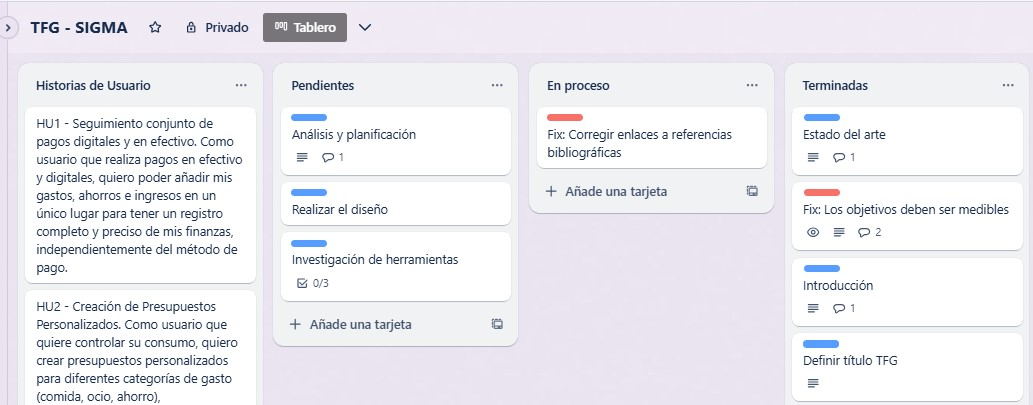
\includegraphics[width=\linewidth]{imagenes/tablero_kanban.jpg}
    \caption{Captura de pantalla del tablero kanban en \textit{Trello}.}
    \label{fig:tablero_kanban}
\end{figure}


\section{Costes}
En este capítulo se describen los recursos y materiales usados en el desarrollo del proyecto, junto con los costos asociados a cada uno de ellos.

\subsection{Recursos humanos}

En el desarrollo de la aplicación web \textit{SIGMA}, se ha contado con un desarrollador que ha hecho también las labores de diseño para la interfaz y redacción de este documento.

\subsection{Hardware y software}
Como recursos materiales, han sido utilizados un ordenador personal portátil y un monitor (Tabla \ref{tab:costes-hardware}),
propiedad del desarrollador, los cuales han sido de gran utilidad para las tareas de diseño y desarrollo al permitir el visionado de diferentes recursos simultáneamente.

\begin{table}[H]
    \begin{center}
    \begin{tabular}{| l | c | c | c |}
        \hline
        \textbf{Hardware} & \textbf{Coste} \\ \hline
        Acer Extensa 2511 & 589\euro \\
        Monitor LG & 132,68\euro \\ \hline
        \textbf{Coste total hardware}: & \textbf{721,68\euro} \\ \hline
    \end{tabular}
    \caption{Coste de materiales hardware.}
    \label{tab:costes-hardware}
    \end{center}
\end{table} 

Para desarrollar este proyecto no se ha usado ningún software ni biblioteca de pago con el propósito de reducir costes, por lo que el software externo no incrementa el coste final. Por otro lado, el coste del hardware anteriormente mencionado, viene condicionado por la vida útil estimada de los dispositivos. En el caso de un ordenador portátil y un monitor, se estiman entre 5 y 7 años (en buenas condiciones)\cite{tecfys2023}.
\begin{equation}
    \textbf{Coste Anual} = \frac {\text{Coste Hardware}}{\text{5 años}} = \text{144,336 €/año}
\end{equation}

\begin{equation}
    \textbf{Coste Mensual} = \frac {\text{Coste Anual}}{\text{12 meses}} = \text{12,03 €/mes}
\end{equation}

\begin{equation}
    \textbf{Materiales x N Meses} = \text{Coste Mensual/mes} \times \text{8 meses} = \text{96,224 €}
\end{equation}

\subsection{Presupuesto sobre profesionales implicados}
En esta sección se detallarán los costos del proyecto. Se considerará el perfil de un puesto junior de desarrollador \textit{fullstack}, cuyo salario anual oscila entre los 17.000€ y 22.000€ \cite{glassdoor2024}.
Teniendo en cuenta que la implementación ha tomado un tiempo aproximado de 370 horas, se puede calcular un coste estimado del salario del desarrollador, el cual se detalla a continuación:

\begin{equation}
    \textbf{Salario medio fullstack junior} =  \frac {\text{19.500 €/año} }{ \text{12 meses}} = \text{1.625 €/mes}
\end{equation}

El salario por hora se calcula dividiendo el salario mensual entre 160 horas, que es el promedio de horas laborales al mes:

\begin{equation}
    \textbf{Salario por hora} = \frac {\text{1.625 €/mes}}{160 \text{ horas}} = \text{10,16 €/hora}
\end{equation}

Teniendo en cuenta las 370 horas de trabajo, se puede calcular el coste total del salario:

\begin{equation}
    \textbf{Coste total salario} = \text{370 horas} \times \text{10.16 €/hora} = \text{3.757,81 €}
\end{equation}

Para el diseño, se tendrá en cuenta el perfil de un diseñador gráfico, cuyo salario medio es de unos 18.180 € \cite{glassdoor-dis-grafico-2024}. Teniendo en cuenta que el diseño ha supuesto un aproximado de 30 horas. Partiendo de esta información, se puede calcular el coste total del salario del diseñador, el cual se detalla a continuación:

\begin{equation}
    \textbf{Salario medio diseñador gráfico} =  \frac {\text{18.180 €/año} }{ \text{12 meses}} = \text{1,515 €/mes}
\end{equation}

El salario por hora se calcula dividiendo el salario mensual entre 160 horas, que es el promedio de horas laborales al mes:

\begin{equation}
    \textbf{Salario por hora} = \frac {\text{1,515 €/mes}}{160 \text{ horas}} = \text{9,47 €/hora}
\end{equation}

Teniendo en cuenta las 30 horas de trabajo, se puede calcular el coste total del salario del diseñador:

\begin{equation}
    \textbf{Coste salario} = \text{30 horas} \times \text{9,47 €/hora} = \text{284,06 €}
\end{equation}

\subsection*{Total}

Sumando los costes asociados a los salarios y materiales usados, se obtiene el coste total aproximado del proyecto (representado en la Tabla \ref{tab:coste-total}).

\begin{table}[H]
    \begin{center}
    \begin{tabular}{| l | c | c | c |}
        \hline
        \textbf{Entidad} & \textbf{Coste} \\ \hline
        Desarrollador & 3.757,81\euro \\
        Diseñador  & 284,06\euro \\ \hline
        Hardware
        \textbf{Coste total}: & \textbf{4.041,87\euro} \\ \hline
    \end{tabular}
    \caption{Coste de materiales hardware.}
    \label{tab:coste-total}
    \end{center}
\end{table} 

	\input{secciones/05_diseño}

	\chapter{Implementación}

La implementación del software se ha dividido en hitos. Estos, han sido definidos en Github
y cada uno de ellos contiene un grupo de \textit{issues} que se corresponden con las distintas
mejoras que se han ido incorporando al software a lo largo de su desarrollo.\\



	\chapter{Conclusiones y trabajos futuros}

\section{Conclusiones}

CONCLUSIONES: Visión comercial?
En la actualidad, cada vez son más los comercios que ofrecen la posibilidad de recibir 
el ticket en formato digital. En un futuro probablemente todos los tickets serán 
digitales para reducir el impacto ambiental del uso del papel y abaratar costes.

Por lo que se incluirá en la aplicación la opción de escaneo de tickets digitales.

	
	\newpage
	\bibliography{bibliografia}
	\bibliographystyle{plain}
	
\end{document}
